\section{Stochastic Potential Games}
\label{sec:spg}

In this section we aim to answer three questions. First, is the class of SPGs distinct from SGPGs? In other words, are there really SPGs that do not have global potential functions? The answer is yes, and we will provide a simple example in this section. Second, to what extent are SPGs applicable in the real world? We will answer this question by examining modular dynamics further, and leveraging the equivalence between potential games and congestion games to examine a "realistic" subclass of SPGs, which we call {\em routing/construction games}. Finally, we will discuss some properties of the set of Nash equilibrium in SPGs.

Let's begin with an example of an SPG that has no global potential function.

\begin{eg}
Consider a 2-player stochastic game $\GG$ with 3 states: $s_1$, $s_2$, and $s_3$. We will call the corresponding stage games $G_1$, $G_2$, and $G_3$ for ease of notation. Episodes of the game always start in $s_1$. Both players have two actions, $a$ and $b$, in each state. The stage games in $s_1$ and $s_3$ are trivial, that is, all actions yield zero utility for both players. The stage game in $s_2$ is given by the following bimatrix:

\[
\begin{blockarray}{ccc}
 & a & b \\
\begin{block}{c(cc)}
  a & 4,2 & 2,2 \\
  b & 2,1 & 2,3 \\
\end{block}
\end{blockarray}
 \]

Finally, the transition probabilities are

$$
P_{12} = 
\begin{pmatrix} 
0 & 0.5 \\
0.5 & 1 
\end{pmatrix}
$$

and then necessarily

$$
P_{13} =
\begin{pmatrix} 
1 & 0.5 \\
0.5 & 0 
\end{pmatrix}
$$

It is straightforward to see that these transition probabilities are modular. $G_{1}$ and $G_{3}$ are trivially potential games with potential function $\phi \equiv 0$. $G_{2}$ is a potential game with potential function:

\[
\begin{blockarray}{ccc}
 & a & b \\
\begin{block}{c(cc)}
  a & 0 & 0 \\
  b & -2 & 0 \\
\end{block}
\end{blockarray}
 \]


Since all stage games are potential games and the dynamics are modular, $\GG$ is an SPG. Now, let
\begin{align*}
&\pi^1 = \pi^2 = [a,a,a] \\
&\tilde{\pi}^1 = [b,a,a] \\
&\tilde{\pi}^2 = [a,b,a]
\end{align*}

Here we use the notation $\left[x, y, z \right]$ as shorthand for the deterministic player behavior:

\begin{center}
"Take action $x$ in state $s_1$, action $y$ in state $s_2$, and action $z$ in state $s_3$."
\end{center}

It is a simple exercise to calculate the value difference of the following joint behaviors:

\begin{align*}
&V^1_{s_1}(\tilde{\pi}^1, \pi^2) - V^1_{s_1}(\pi^1, \pi^2) = 2 \\
&V^2_{s_1}(\tilde{\pi}^1, \tilde{\pi}^2) - V^2_{s_1}(\tilde{\pi}^1, \pi^2) = 1 \\
&V^2_{s_1}(\pi^1, \tilde{\pi}^2) - V^2_{s_1}(\pi^1, \pi^2) = 1 \\
&V^1_{s_1}(\tilde{\pi}^1, \tilde{\pi}^2) - V^1_{s_1}(\pi^1, \tilde{\pi}^2) = 1 \\
\end{align*}

Because these returns do not commute (ie $2+1 \neq 1+1$) there cannot exist a global potential function. In the next section we will describe all of the constraints associated with SGPGs and write them down explicitly. At that point, we will be able to more clearly identify why the above example has no global potential function. For now we simply point out that in the above example the commutativity issue arose when we changed the players' actions at different states, namely $s_1$ and $s_2$. In particular, these states occur at different layers in the finite MDP over joint actions.

\label{eg:spgnotsgpg}
\end{eg}


\subsection{Modular dynamics with a view towards applications}

In the previous subsection we confirmed that SPGs are a distinct class of stochastic games, and that they may not have global potential functions. In this section we will explore the definition of SPGs and characterize modular dynamics in a way that suggests possible real-world applications. We will end this section by identifying a subclass of SPGs, which we call {\em routing/construction games} which may be of interest in engineering and economics applications.

Recall that a stochastic game $G$ has modular dynamics if for all state pairs $s$ and $s'$, joint action $a$, players $i$ and $j$ with alternative actions $b^i$ and $b^j$, the following equation holds:

\begin{equation}
P_{ss'}(a) + P_{ss'}(\asub{a}{b^ib^j}) = P_{ss'}(\asub{a}{b^i}) + P_{ss'}(\asub{a}{b^j})
\label{eq:modular2}
\end{equation}

This equation defines the transition probabilities of SPGs in terms of constraints. The following sequence of results transforms this into a constructive characterization of transition probabilities.

\begin{proposition}
If $\GG$ has modular dynamics then for any player $i$, states $s$ and $s'$,  joint actions $a$ and $b$ with $a^i = b^i$, and player action $c^i$,

$$
P_{s'}(a) - P_{ss'}(\asub{a}{c^i}) = P_{s'}(b) - P_{ss'}(\asub{b}{c^i}) 
$$
\end{proposition}

\begin{proof}
We know this is true when $a^{-i}$ and $b^{-i}$ differ by a single player's action since modular dynamics tells us that
$$
P_{ss'}(a) - P_{ss'}(\asub{a}{b^i}) = P_{ss'}(\asub{a}{b^j}) - P_{ss'}(\asub{a}{b^ib^j})
$$

For general $a$ and $b$ with $a^i = b^i$, we simply chain together single action changes, maintaining equality throughout the process, ie

\begin{align*}
P_{ss'}(a) - P_{ss'}(\asub{a}{c^i}) &= P_{ss'}(\asub{a}{b^1}) - P_{ss'}(\asub{a}{c^ib^1}) \\
&= P_{ss'}(\asub{a}{b^1b^2}) - P_{ss'}(\asub{a}{c^ib^1b^2}) \\
\vdots \\
&= P_{ss'}(\asub{a}{b^1\cdots b^{i-1}b^i b^n}) - P_{ss'}(\asub{a}{b^1\cdots b^{i-1}b^{i+1} b^nc^i}) \\
&= P_{ss'}(b) - P_{ss'}(\asub{b}{c^i})
\end{align*}
\end{proof}

\begin{lem}
If $\GG$ is a stochastic game with modular dynamics then for any pair of states $s$ and $s'$, there exists a {\em nonnegative} constant $c_{ss'}$ and {\em nonnegative} functions
$$
f^i_{ss'} : \AA^i \rightarrow \R
$$

for each player such that

$$
P_{ss'}(a) = c_{ss'} + \sum_{i=1}^n f^i_{ss'}(a^i)
$$
\end{lem}

\begin{proof}

Fix player $i$ and joint action $b$ such that

$$
b^i \in \text{argmin}_{b^i} P_{ss'}(b^i, b^{-i})
$$

Define the following functions


\begin{eqnarray*}
f^i_{ss'}(a^i) &:=& P_{ss'}(a^i, b^{-i}) - P_{ss'}(b^i, b^{-i}) \\
g^i_{ss'}(a^{-i}) &:=& P_{ss'}(b^i, a^{-i})
\end{eqnarray*}


Notice that by construction 
$$
P_{ss'}(a^i, a^{-i}) = f^i_{ss'}(a^i) + g^i_{ss'}(a^{-i})
$$

Since we can do this for all players, we can decompose $P_{ss'}(a)$ as

$$
P_{ss'}(a) = c_{ss'} + \sum_{i=1}^n f^i_{ss'}(a^i)
$$

Furthermore, since $b^i \in \text{argmin}_{b^i} P_{ss'}(b^i, b^{-i})$, all of the functions $f^i_{ss'}$ are nonnegative, and reach their minimum value of $0$ when $a^i = b^i$. Note that there are possibly other minima.

Finally, we need to show that $c_{ss'}$ is nonnegative. But, based on our previous statement, we can certainly choose a joint action $c$ such that all of the functions $f^i_{ss'}$ are simultaneously zero. Then

$$
P_{ss'}(c) = c_{ss'}
$$
\end{proof}



\begin{thm}
Let $\GG$ be a stochastic game. Then $\GG$ has modular dynamics if and only if for every state $s$ there exist state dependent player weights $w^i_s$, action-conditional probability distributions over next states $\{p^i_{ss'}(a^i) \}$, and "natural weights" $w^0_{ss'}$,  such that

$$
P_{ss'}(a) = w_{ss'}^0 + \sum_{i} w^i_s p^i_{ss'}(a^i)
$$

\begin{proof}

Suppose $\GG$ has modular dynamics. Then by the previous lemma we have the decomposition

$$
P_{ss'}(a) = c_{ss'} + \sum_{i=1}^n f^i_{ss'}(a^i)
$$

where $c_{ss'}$ and $f^i_{ss'}(a^i)$ are all nonnegative. Since $P_{ss'}(a)$ is a probability distribution over next states $s'$, 

$$
\sum_{s'} \sum_{i=1}^n f^i_{ss'}(a^i) = \sum_{s'} P_{ss'}(a) = 1
$$

Suppose we fix a player $j$ and alter their action to $b^j$ while keeping all other actions fixed. Then
$$
\sum_{s'} \sum_{i=1}^n f^i_{ss'}(a^i) = 1 = \sum_{s'} f^j_{ss'}(b^j) + \sum_{s'} \sum_{i=1, i \neq j}^n f^i_{ss'}(a^i)
$$

The terms not related to player $j$ cancel on both sides leaving

$$
\sum_{s'} f^j_{ss'}(a^j) = \sum_{s'} f^j_{ss'}(b^j)
$$

This equality holds for any pair of player $j$ actions and so it defines an action independent quantity $w_{s}^j := \sum_{s'} f^j_{ss'}(a^j)$. For a given action $b^j$ let
$$
p_{ss'}(b^j) = \dfrac{f^j_{ss'}(b^j)}{w_s^j}
$$

This defines a probability distribution over next states $s'$ that depends on the current state $s$ and player action $b^j$. Letting $w^0_{ss'} = c_{ss'}$ yields
$$
P_{ss'}(a) = w_{ss'}^0 + \sum_{i} w^i_{s} p^i_{ss'}(a^i)
$$


Now we need to show the reverse implication. Suppose $G$ has transition probabilities that can be decomposed as
$$
P_{ss'}(a) = w_{ss'}^0 + \sum_{i} w^i_{s} p^i_{ss'}(a^i)
$$

Let $b^i$ and $b^j$ be alternative actions for players $i$ and $j$. Then

$$
P_{ss'}(a) - P_{ss'}(\asub{a}{b^i}) = w^{i}_{s}p^i_{ss'}(a^i) - w^{i}_{s}p^i_{ss'}(b^i)
$$

and similarly

$$
P_{ss'}(\asub{a}{b^j}) - P_{ss'}(\asub{a}{b^ib^j}) = w^{i}_{s}p^i_{ss'}(a^i) - w^{i}_{s}p^i_{ss'}(b^i)
$$

So

\begin{align*}
P_{ss'}(a) - P_{ss'}(\asub{a}{b^i}) = P_{ss'}(\asub{a}{b^j}) - P_{ss'}(\asub{a}{b^ib^j}) \\
P_{ss'}(\asub{a}{b^j}) + P_{ss'}(\asub{a}{b^j}) = P_{ss'}(a) + P_{ss'}(\asub{a}{b^ib^j})
\end{align*}

Therefore $\GG$ has modular dynamics.
\end{proof}

\label{thm:weightvote}
\end{thm}


The above theorem allows us to describe the mechanics of an SPG $\GG$ in plain language as follows. In a give state, players are endowed with "voting shares" specified by the $w^i_s$'s. The various actions that a player $i$ can take determine how that player's voting share is distributed across next states. A priori, player $i$ does not have full control in distributing $w^i_s$ across next states, but rather is constrained by their action set. For example, suppose that the action set $\AA^i_s$ of a layer $k$ state $s$ exactly corresponds to $\SS_{k+1}$, the set of layer $k+1$ states. So an element of $\AA^i_s$ can be identified with a next state $s'$. Furthermore, suppose that $p^i_{ss'}(s') = 1$. In this kind of game, players can only distribute their voting share unilaterally on a single next state and cannot "manage risk" by placing voting shares on multiple next states.


In addition to each player having a voting share, nature is also endowed with a state-dependent voting share $w^0_s = \sum_{s'} w^0_{ss'}$. In the extreme case $w^0_s = 1$, in which case players have {\em no} control on transition probabilities and should therefore act myopically in state $s$.

As a first example, let's reexamine \ref{eg:spgnotsgpg}. There are two state dependent weights

\begin{align*}
w^1_{1} = 0.5 \\
w^2_{1} = 0.5
\end{align*}

The natural weights are all zero. Furthermore the probability distributions are simply
\begin{align*}
p^i_{12}(a) = 0 \\
p^i_{13}(a) = 1
\end{align*}

and

\begin{align*}
p^i_{12}(b) = 1 \\
p^i_{13}(b) = 0
\end{align*}


For both players $i = 1$ and $i = 2$. This is an example not only of an SPG in general, but of the special case noted in the paragraph above. Namely, each player has two actions that correspond exactly with the number of next states. Action $a$ casts a vote for state $s_3$ and action $b$ casts a vote for $s_2$. Both players have equal voting shares, and the natural weights are zero. 

\subsection{Routing/construction games}

In the pioneering paper on potential games \cite{monderer1996potential}, Monderer and Shapley show that the class of potential games is equivalent to the class of {\em congestion games}. They do so through explicitly constructing potential functions for arbitrary congestion games, and conversely constructing a congestion game out of an arbitrary potential function. The link between congestion games and potential functions can be traced further back to the work of Rosenthal \cite{rosenthal1973class} where congestion games are defined and the existence of pure Nash equilibrium is shown through the construction of a potential function. 

A congestion game arises when a set of {\em homogeneous} players have to select from a set of resources, and where the payoff of a player depends on the number of players selecting each resource \cite{monderer1996potential}. Congestion games form a natural model for traffic routing, both in the context of automobile traffic \cite{wang2013distributed} and internet packet traffic \cite{gibbens1999resource}. Below is a precise definition of a congestion game:

\begin{mydef}
A (finite) congestion game consists of the following data:
\begin{enumerate}
    \item A (finite) set of $n$ players
    \item A (finite) set of resources $M$
    \item For each player $i$ a (finite) set of actions $\AA^i$ where each action $a \in \AA^i$ corresponds to a subset of $M$.
    \item For each resource $m \in M$ a delay function $d_m: \mathbb{N} \rightarrow \mathbb{R}$
\end{enumerate}

For a joint action $a$ and resource $m$ let $C_m(a)$ be the number of player actions that contain resource $m$. The payoff of player $i$ is defined to be

\begin{equation}
    u^i(a) = \sum_{m \in a^i} d_m(C_m(a))
\end{equation}

\end{mydef}

Routing games form a special subclass of congestion games. A routing game is a congestion game where the resources $M$ consist of edges in a fixed graph $\Gamma$ and the actions of player $i$ consist of paths in the graph that all have the same starting and ending location. The iterated version of this problem models the strategic aspect of morning commutes. Each day drivers must decide amongst multiple routes between their home and workplace. These routes have different trip times that are dependent on the number of other players utilizing the roadways.

\begin{example}

\begin{figure}
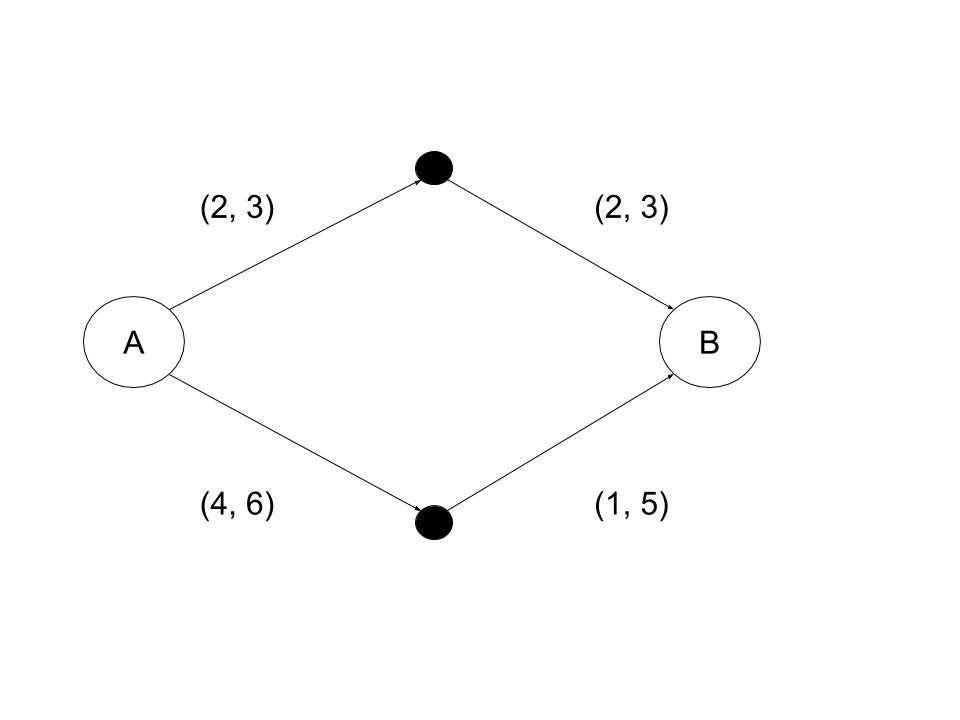
\includegraphics[scale=0.2]{images/simple_congestion_game.jpg}
\caption{A simple routing game.}
\label{fig:cong}
\end{figure}

Figure \ref{fig:cong} shows a simple two player congestion game. There are two players, and they each need to travel from vertex $A$ to vertex $B$. The edges are labelled with pairs of numbers $\left(a, b\right)$ where $a$ is the delay cost when one player utilizes the edge and $b$ is the delay cost when two players utilize the edge. There are two pure Nash equilibria in this game. Either player one takes the upper route and player two takes the lower route or vice versa. 
\end{example}


\subsubsection{Connecting routing games and SPGs} Recall that the first property of SPGs is that each stage game is a potential game. Since every potential game is equivalent to a congestion game, we can instead think of the SPG as being made up of a collection of congestion games with modular transition probabilities. A priori there may be no "physical" relationship between the stage congestion games in an SPG. Below we describe {\em routing/construction games} which are a subset of SPGs in which the stage congestion games (specifically, routing games) are connected in a physical way.

% One advantage of viewing potential games as congestion games is that a congestion game has a natural description of state given by its graph $\mathcal{G}$ and the set of delay functions $d_m$. 

In the traditional routing game story, one imagines a network of roads, and a set of commuters with various start and end locations. Each road has an associated delay function which relates the number of commuters on a road to the expected time it will take a given commuter to traverse that road. This can depend on a number of road characteristics such as speed limit, lanes, and road quality. It is the "job" of commuters (players) to select how to {\em route} themselves.

We are going to modify this story by adding in a new actor which we will call "the government". At each timestep, the government observes the strategy of commuters and elects to take on {\em construction} projects to fix roads, add lanes, etc. based which roads the commuters chose at the last timestep. These choices are reflected in modifications to the road delay functions. It is natural to assume that the government is more likely to fix roads that are used by a large number of drivers, and this is where the "voting" interpretation of modular dynamics is employed. In order to fit the SPG model to this situation, the government must modify the roads probabilistically. We provide the full definition of routing/construction games below. 



\begin{mydef}
An $n$-player routing/construction game $\G$ consists of a directed graph $\Gamma = (V, E)$. The graph has an initial set of delay functions 
$$
d^0_{e} : \{1, \ldots, n\} \rightarrow \mathbb{R}
$$ 

\noindent for each $e \in E$ which defines an initial stage routing game. It is also equipped with "construction" functions

$$
c_{e}(d_{e}, b): \mathbb{R}^n \times \{0,1\} \rightarrow \mathbb{R}^n
$$

\noindent which describe how the delay functions change from state to state. At state $s$, let $d^s_e$ denote the delay function on edge $e$. From this state, the government will be able to strengthen one edge, and all other roads will decay. 

Suppose players select joint action $a$. This action defines a probability distribution over {\em edges} as follows. Each player has identical voting share $w^i_{s} = \frac{1}{n}$. If player $i$'s action is made up of a subset of edges $e_1^i, \ldots, e_r^i$, then their corresponding vote is a uniform distribution over these edges.

A sample is drawn from this distribution. For the selected edge, the new delay function is

$$
d_e^{s'} = c_{e}(d_{e}^{s}, 1)
$$

and for all other edges $f$, the new delay function is 

$$
d_f^{s'} = c_{f}(d_{f}^{s}, 0)
$$

The game $\GG$ proceeds for a fixed number of layers $k$ and then terminates.

Intuitively, construction on an edge should {\em reduce} the values of the delay function while decay should {\em increase} values of the delay function, so that

$$
d_e^{s'} = c_{e}(d_{e}^{s}, 1) \leq d_{e}^s \leq d_e^{s'} = c_{e}(d_{e}^{s}, 0)
$$

\end{mydef}

By construction, routing/construction games are SPGs since we have described their transition dynamics in terms of state and player dependent weights and action conditional probability distributions. 


\subsection{Equilibria}

The set of Nash equilibria in a potential games has two immediately interesting features. First, every potential games admits at least one {\em pure} Nash equilibrium. Second, potential games admit further specialized equilibria which are called "potential maximizing equilibria". These are joint behaviors that maximize the potential function. In some applications, the potential function is interpreted as a welfare function, and one desires to find learning algorithms that converge to potential maximizing behavior. We say that a learning algorithm has "equilibrium selection properties" if it is guaranteed to converge to a certain subset of Nash equilibria. So, an algorithm that converges to the set of potential maximizing equilibria in a potential game has an equilibrium selection property. Log linear learning \cite{marden2012revisiting, young1993evolution} is an example of such a learning algorithm, and we will discuss it further in the next chapter.

\begin{mydef}

Let $G$ be an SPG. A joint behavior $\pi$ is called a {\em simultaneously potential maximizing} if, for each state $s$, the joint behavior $\pi_s$ maximizes the potential function that has utilities

\begin{equation}
    u^i_s(a) + \sum_{s'} P_{ss'} V^i_{\pi}(s')
\end{equation}

\end{mydef}


The three main results of this section are

\begin{thm}
Every stochastic potential game admits a pure Nash equilibrium.
\end{thm}

\begin{thm}
Every simultaneously potential maximizing equilibrium is a Nash equilibrium.
\end{thm}

\begin{thm}
Every stochastic potential game admits a simultaneously potential maximizing equilibrium.
\end{thm}

We will prove all of these results together.

\begin{proof}
Let $G$ be an $n$-player stochastic potential game. As usual denote the state layers by $\SS_1, \ldots, \SS_T$, the stage potential games by $G_s$ with potential $\phi_s$ and utilities $u^i_s$.

We will construct a pure simultaneously potential maximizing Nash equilibrium $\pi$ by a backwards iterative method through the layers of $G$.

First, for each state $s \in \SS_T$ let $a_s$ be a pure potential maximizing Nash equilibrium for the stage game $G_s$. Set $\pi_s \coloneq a_s$ and then $V^i_{\pi}(s) = u^i_s(a_s)$. Note that we haven't fully defined $\pi$ yet, but it is okay to talk about $V^i_{\pi}(s)$ for states $s \in S_T$ since we have described the behavior of $\pi$ at layer $T$.

Next, for each state $s \in \SS_{T-1}$ consider the continuation game $G_s(V^i_{\pi})$ with utilities

$$
u^i_s(a) + \sum_{s' \in \SS_{T}}P_{ss'}(a)V^i_{\pi}(s')
$$

Since $G$ is a stochastic potential game, each $G_s(V^i_{\pi})$ is a potential game and hence admits a pure potential maximizing Nash equilibrium $a_s$. For the states in $\SS_{T-1}$ set $\pi_s \coloneq a_s$ and then $V^i_{\pi}(s) = u^i_s(a_s) + \sum_{s' \in \SS_T}P_{ss'}(a_s)V^i_{s'}$.

Iterating this process, for each state $s \in S_j$ consider the continuation game $G_s(V^i_{\pi})$ with utilities

$$
u^i_s(a) + \sum_{s' \in \SS_{T}}P_{ss'}(a)V^i_{\pi}(s')
$$

This game admits a pure Nash equilibrium $a_s$. We set $\pi_s \coloneq a_s$ for all $s \in \SS_j$ and $V^i_{\pi} = u^i_s(a_s) + \sum_{s' \in \SS_T}P_{ss'}(a_s)V^i_{\pi}(s')$. 


Eventually this process terminates, at which point it defines a pure joint strategy in every state, that is, a pure joint behavior $\pi$. By construction it is clear that $\pi$ is simultaneously potential maximizing. Finally, we need to show that $\pi$ is a Nash equilibrium.

Fix a player $i$ whose behavior under $\pi$ is $\pi^i$ and consider an alternative behavior $\tau^i$. Let $t_0$ be the last layer where $\pi^i$ and $\tau^i$ differ. That is, the largest $t_0$ such that there exists $s_0 \in \SS_{t_0}$ with$\pi^i_{s_0} \neq \tau^i_{s_0}$. Then the behaviors $\pi^i$ and $\asub{\pi}{\tau^i}$ correspond to strategies in the game $G_{s_0}(z(t_0+1))$. But, since we know that $\pi_s$ is a Nash equilibrium for the game $G_{s_0}(V^i_{\pi})$, it must be the case that

$$
u^i_s(\pi_s) + \sum_{s' \in \SS_{t_0+1}} P_{ss'}(\pi_s)V^i_{\pi}(s') \geq u^i_s(\asub{\pi_s}{\tau^i}) + \sum_{s' \in \SS_{t_0+1}} P_{ss'}(\asub{\pi_s}{\tau^i})V^i_{\pi}(s')
$$

Therefore $\pi$ is a Nash equilibrium.


\end{proof}

